\documentclass[aps,onecolumn, notitlepage, longbibliography]{revtex4-1}
%\linespread{2}

\usepackage{amsmath}
\usepackage{bm}
\usepackage{bbm}
\usepackage{graphicx}% Include figure files
\usepackage{dcolumn}
\usepackage{bm}% bold math
\usepackage[colorlinks=true,bookmarks=false,citecolor=blue,linkcolor=blue,hyperfootnotes=true,urlcolor=blue]{hyperref}
\usepackage{color}
\usepackage{comment}
\usepackage{todonotes}
\usepackage{sidecap}

\begin{document}

\title{Notes on the RIXS cross-section, azimuthal dependence and polarization dependence}


%\author{G. Fabbris}
%\author{M. P. M. Dean}
%\email{mdean@bnl.gov}


% user macros
\def\mathbi#1{\ensuremath{\textbf{\em #1}}}
\def\Q{\ensuremath{\mathbi{Q}}}
\def\LNO{LaNiO$_3$}
\newcommand{\angstrom}{\mbox{\normalfont\AA}}
\date{\today}

\newcommand{\ket}[1]{\left|{#1}\right>}
\newcommand{\bra}[1]{\left<{#1}\right|}
\newcommand{\abs}[1]{\left|{#1}\right|}

% insert suggested PACS numbers in braces on next line
\pacs{74.70.Xa,75.25.-j,71.70.Ej}
% insert suggested keywords - APS authors don't need to do this
%\keywords{}
%
%\maketitle must follow title, authors, abstract, \pacs, and \keywords
\maketitle

In these notes we consider the case of direct or ``operator'' RIXS relevant to experiments in which the measured intensity is dominated by dipole transitions from a $2p$ core state into a $d$ character valance orbital. Most results are taken from Ref.~\cite{Ament2011} with some additional explanations and emphasis. The probability of incident photons with wavevector ${\bf k}$, polarization ${\bf \epsilon_k}$ and energy $\hbar \omega_{\bf k}$ being scattered to states ${\bf k}^\prime$, ${\bf \epsilon_k}^\prime$ and $\hbar \omega_{\bf k}^\prime$ is described by the double differential cross section
\begin{eqnarray}
I(\omega,{\bf k},{\bf k}',{\bm \epsilon},{\bm \epsilon}') &=& r_e^2m^2\omega_{{\bf k}'}^3\omega_{\bf k} \sum_{\tt f}|{\cal F}_{fg}({\bf k}, {\bf k}^\prime, {\boldsymbol \epsilon}, {\boldsymbol \epsilon}^\prime, \omega_{\bf k}, \omega_{{\bf k}^\prime})|^2  \nonumber \\
&& ~~~\times  \delta (E_g-E_f+\hbar \omega) ,
\label{KramersH}
\end{eqnarray}
 where $r_e = \frac{1}{4\pi \epsilon_0} \frac{e^2}{mc^2}$ the classical electron radius. The scattering amplitude from the ground state $\ket{g}$, through intermediate state $\abs{n}$ to the final state $\bra{f}$ is given by
\begin{eqnarray}
&& {\cal F}_{fg}({\bf k}, {\bf k}^\prime, {\boldsymbol \epsilon}, {\boldsymbol \epsilon}^\prime, \omega_{\bf k}, \omega_{{\bf k}^\prime}) =  \sum_n
	 \frac{\bra{f} {\cal D}'^\dagger  \ket{n} \bra{n} {\cal D} \ket{g}}{E_g+\hbar \omega_{\bf k}-E_n+i\Gamma_n},
\label{eq:K-H}
\end{eqnarray}
where $E_g$ and $E_n$ are the energies of $\ket{g}$ and $\abs{n}$ and $\Gamma_n$ is the inverse core hole lifetime. Under the dipole approximation we can write
\begin{equation}
  {\cal D}={\boldsymbol \epsilon} \cdot {\bf D} ~~~{\rm with} ~~~~
 {\bf D}= \sum_{i=1}^N e^{i{\bf k} \cdot {\bf R}_i} {\bf r}_i,
 \label{eq:transoper}
\end{equation}
where ${\bf R}_i$ is the position of the ion to which electron $i$ is bound and ${\bf r}_i$ is the position operator. We now note that the operator ${\cal D}$ is a three component object that depends on the symmetry of the atom. This is made explicit by adding a subscript to define $D_\alpha$ where $\alpha=-1,0,1$ such that
\begin{equation}
 {\cal F}_{\alpha^\prime\alpha} =  \sum_n
	 \frac{\bra{f} D_{\alpha^\prime}^\dagger  \ket{n} \bra{n} D_\alpha \ket{g}}{E_g+\hbar \omega_{\bf k}-E_n+i\Gamma_n}.
\label{Falphaalpha}
\end{equation}
In a Cartesian basis $\alpha$ could index the three perpendicular directions in space $\alpha=x,y,z$ or, alternatively circular left, linear and circular right light. In any appropriate orthogonal basis, dipole RIXS process can be described in terms of $3\times3=9$ fundamental scattering amplitudes \cite{Ament2011}. These can be conveniently represented in terms of a matrix 
\begin{equation}
 {\cal F}_{\alpha^\prime\alpha} =
  \begin{pmatrix}
    F_{-1-1} & F_{-10}  & F_{-11}  \\
    F_{0-1} & F_{00}  & F_{01}  \\
   F_{1-1} & F_{10}  & F_{11}
  \end{pmatrix} .
\end{equation}
Note that these elements do not interfere with one another (as can be seen by examining Eq.~\ref{KramersH}) because they represent distinct paths through the intermediate state.

\section{Azimuthal dependence}
\begin{figure*}
    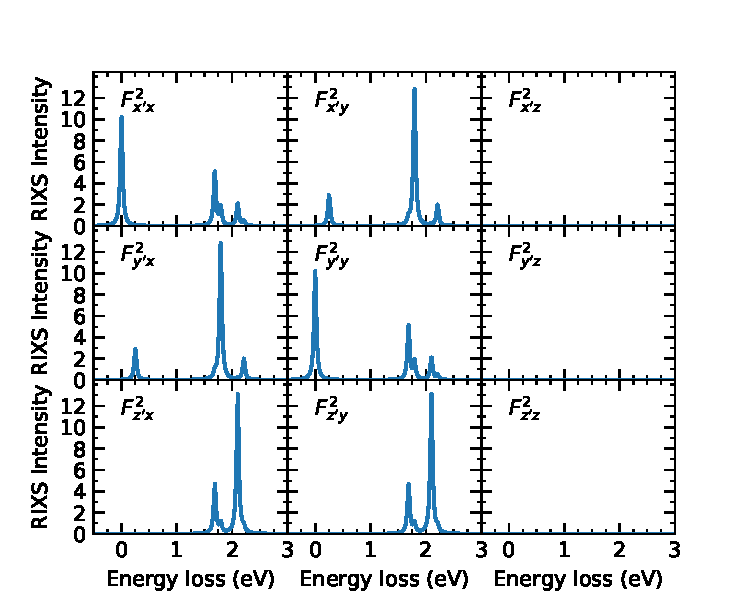
\includegraphics{Cu_RIXS.pdf}
    \caption{The different components of the RIXS cross section for a Cu $d^9$ ion in a tetragonal crystal field.}
    \label{Cu_RIXS_spectra}
\end{figure*}

\begin{figure}
    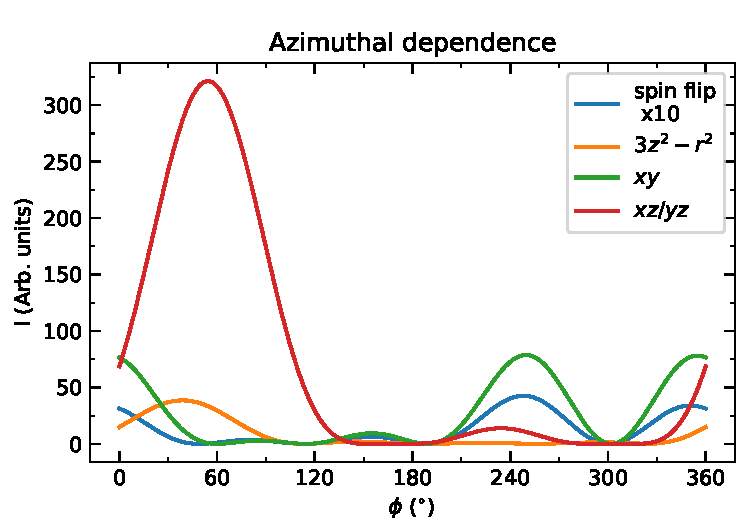
\includegraphics{azimuthal.pdf}
    \caption{The azimuthal dependence RIXS cross section for a Cu $d^9$ ion in a tetragonal crystal field. The starting condition at $\phi=0^{\circ}$ has scattering angle $2\theta=130^{\circ}$ and incident angle $\theta_i=120^{\circ}$ and $\pi$ polarized light.  \label{azimuthal}}
\end{figure}

With this background in place, we can make some comments about azimuthal dependence. Measuring the azimuthal dependence of the scattering is a very popular technique in resonant x-ray scattering experiments. This can be traced back to an expression by Hannon et al.\ in Ref.~\cite{Hannon1988} that relates the magnetic scattering amplitude from a site with magnetization direction $\bm{\hat{m}}$ a to a simple cross product of the incident and scattered polarizations 
 \begin{equation}
 {\cal F}_{\alpha^\prime\alpha} = \epsilon^\prime \times \epsilon \cdot \bm{\hat{m}}
\end{equation}
or in matrix form
 \begin{equation}
 {\cal F}_{\alpha^\prime\alpha} = \epsilon^\prime \cdot
   \begin{pmatrix}
    0 & 1  & -1  \\
    -1 & 0  & 1  \\
   1 & -1  & 0
  \end{pmatrix} 
 \cdot \epsilon 
 \label{cross_product_matrix}
\end{equation}
%\todo[inline]{Is there another symmetry to this object}
Attractive as this expression is, it is only strictly valid in spherical symmetry \cite{Mazzoli2007, Haverkort2010_symmetry, Juhin2014}. In the solid state, however, there is almost always appreciable crystal field interactions -- these are of order 2~eV in typical $3d$ transition metal oxides.  In elastic scattering experiments one usually works with an x-ray beam bandwidth that is comparable to or larger than the magnitude of the crystal field, in which limit, this expression might be an adequate approximation. For RIXS, however, the bandwidth will typically be smaller than the crystal field and one will always directly observe the branching of the different transitions. We can see how this works in practise by computing RIXS under the dipole approximation using the standard multiplet approach. For this, we choose a Cartesian basis
\begin{equation}
 {\cal F}_{\alpha^\prime\alpha} =
  \begin{pmatrix}
    F_{x^\prime x} & F_{x^\prime y}  & F_{x^\prime z}  \\
    F_{y^\prime x} & F_{y^\prime y}  & F_{y^\prime z}  \\
   F_{z^\prime x} & F_{z^\prime y}  & F_{z^\prime z}
  \end{pmatrix} .
\end{equation}
Figure~\ref{Cu_RIXS_spectra} shows the 9 fundamental RIXS channels for a Cu $d^9$ ion in a tetragonal crystal field. All three channels with $z$-polarized incident light are zero, because light with this polarization cannot excite into the $x^2-y^2$ ground state orbital. This breaks the simple cross product rule as can be seen by comparing to Eq.~\ref{cross_product_matrix}. The main point to emphasize, is that unless an azimuthal scan is performed about a high symmetry direction of the crystal it will mix the different components in a rather complicated way as illustrated in the example calculation shown in Fig.~\ref{azimuthal} and it is hard to see a particular advantage of this approach. In most experiments it seems prudent to use calculations to maximize the overall cross-section and cross-section contrast between different channels. 

\section{Polarimetry}
Based on the form of ${\cal F}_{\alpha^\prime\alpha}$ we can make some comments regarding polarimetry. For soft x-rays we can easily generate three independent polarization components in the incident beam. For example, two circular and one linear component. One the scattered side it might initially appear that one must similarly detect three components. However here, we can exploit the fact that at a given scattering angle we know that the electric field along the beam direction is zero. Consequently, if one measures two linear components of the scattered light one can impose three constrains on the scattered polarization. Thus by measuring three scattered components with three different incident polarizations one should be able to obtain all the information contained in a RIXS spectrum \footnote{In some pathological cases one may need to measure different scattering angles, but this is unlikely to present particular problems.}. 

For the case of cuprates the situation, as shown in Fig.~\ref{pol_dep} is particularly simple: the spin flip or magnon excitation is present in $\pi-\sigma$ and $\sigma-\pi$ channels and absent in $\pi-\pi$ and $\sigma-\sigma$ channels and the converse is true for phonons. 

\begin{figure}
    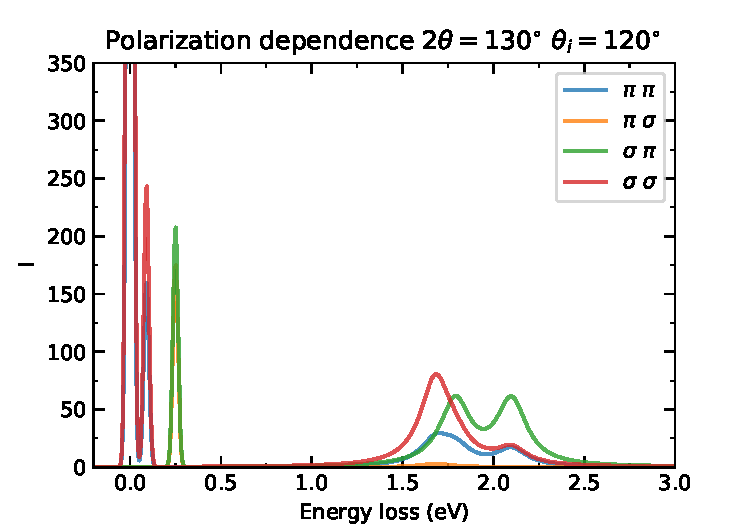
\includegraphics{pol_dep.pdf}
    \caption{The azimuthal dependence RIXS cross section for a Cu $d^9$ ion in a tetragonal crystal field. The starting condition at $\phi=0^{\circ}$ has scattering angle $2\theta=130^{\circ}$ and incident angle $\theta_i=120^{\circ}$ and $\pi$ polarized light as depicted in Fig.~\ref{geometry}. \label{pol_dep}}
\end{figure}

\begin{figure}
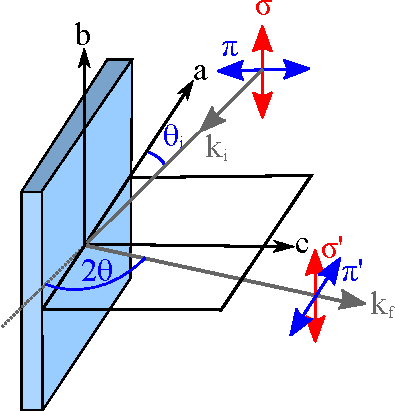
\includegraphics[width=1.7 in]{geometry.pdf}
\caption{RIXS scattering geometry. Linearly polarized x-rays ($\sigma$ or $\pi$) are incident upon the sample at an angle $\theta _i$. The scattered photons with $\sigma^\prime$ or $\pi^\prime$ polarization emitted at $\theta_o$ with respect to the sample surface are collected at $2\theta = 90^\circ$. \label{geometry}}
\end{figure}

%Hill1996
% Haverkort2010_symmetry
%Haverkort2010

\section{Polarization analysis at $2\theta \neq 90^\circ$ }
In practise it is very challenging to produce soft x-ray polarimeters that can completely separate  the different scattered polarization. Consequently, we consider what happens in the case of a polarimeter that operates at $2\theta \neq 90^\circ$ taking some useful results from Detlafs, del Rio and Mazzoli in Ref.~\cite{Detlefs2012}. The polarization state of an isolated wave
\begin{equation}
        {\bf E}(t, {\bf r})
        = \Re \{
                \left(V_{\pi} \epsilon_{\pi} 
                + V_{\sigma} \epsilon_{\sigma}\right)
        \exp \left[ -i(\omega_{\bf k} t - {\bf k}\cdot{\bf r}) \right]
        \}
        \label{el_field}
\end{equation}
is completely defined by the two complex components of the Jones vector,
\begin{equation}
{\bf V} = \left(\begin{array}{c}V_\sigma\\V_\pi\end{array}\right). \end{equation}
A more general x-ray beam composed of an ensemble of independent waves can be partially polarized and can be represented using the coherency matrix
\begin{equation}
{\bf \rho} = 
  \begin{pmatrix}
    \langle V_{\sigma}V_{\sigma}^{\dagger} \rangle  & \langle V_{\sigma}V_{\pi}^{\dagger} \rangle \\
    \langle V_{\pi}V_{\sigma}^{\dagger} \rangle &  \langle V_{\pi}V_{\pi}^{\dagger} \rangle
  \end{pmatrix} .
\end{equation}
The effect of an optical element on this beam can be described by a Jones matrix. For Thomson scattering through an angle $2\theta$ in the kinematic approximation, this matrix is diagonal and scales the components without mixing them
\begin{equation}
{\bf M}_{Th} = R^2
  \begin{pmatrix}
    1  & 0  \\
    0 &  \cos^2(\theta)
  \end{pmatrix} .
\end{equation}
The Jones vector transforms as
\begin{equation}
{\bf V}^\prime = {\bf M}_{Th} \cdot {\bf V} =  \left(\begin{array}{c} V_\pi \\ V_\sigma \cos^2(\theta) \end{array}\right) \end{equation}
under Thomson scattering. The coherency matrix transforms as 
\begin{equation}
{\bf \rho}^\prime = {\bf M}_{Th} \cdot {\bf \rho} \cdot {\bf M}_{Th}^{\dagger} =
  \begin{pmatrix}
    \langle V_{\sigma}V_{\sigma}^{\dagger} \rangle  & \langle V_{\sigma}V_{\pi}^{\dagger}  \rangle \cos^2(\theta) \\
    \langle V_{\pi}V_{\sigma}^{\dagger} \rangle \cos^2(\theta) &  \langle V_{\pi}V_{\pi}^{\dagger} \cos^4(\theta)\rangle
  \end{pmatrix} .
\end{equation}
We plan to calibrate $R^2$ by measuring a known elastic scatter that will produce only $\sigma \sigma$-scattering and to determine $\theta$ mechanically. 

\bibliography{refs}

\end{document}